\documentclass[a4paper,8pt]{beamer}
%\documentclass{beamer}
%\input{embed_video.tex}
\mode<presentation>
%{
  \usetheme{Boadilla}
  % possiblities Singapore, Malmoe, Dresden 
  \setbeamercovered{invisible}
%}
%color setting more or less matching U of A colors
\setbeamercolor*{palette secondary}{use=structure,fg=white,bg=structure.fg!55!black}
\setbeamercolor*{palette tertiary}{use=structure,fg=white,bg=red!50!black}

% Define a sober color theme
\definecolor{mycolor}{RGB}{0,102,204}
\setbeamercolor{item}{fg=mycolor}
\setbeamercolor{section in toc}{fg=mycolor}
\setbeamercolor{footline}{bg=mycolor, fg=white}
\setbeamercolor{headline}{bg=mycolor, fg=white}
\setbeamercolor{title}{fg=mycolor}
\setbeamercolor{author}{fg=mycolor}

%\usetheme{CambridgeUS}
%\usecolortheme{wolverine}
\usepackage[
    backend=biber,
%    style=phys,
%    pageranges=false,
%    biblabel=brackets,
%    chaptertitle=false,
%    articletitle=false,
    maxbibnames=3 %,
%    doi=false, url=false, isbn=false
]{biblatex}
\usepackage[utf8]{inputenc}
\usepackage{graphicx}
\usepackage{bm}
\usepackage{tabularx,booktabs}
\usepackage{subcaption}
\usepackage{hyperref}
\setbeamertemplate{footline}[frame number]
\usepackage{tikz}
\usetikzlibrary{arrows}
\definecolor{myblue}{RGB}{5,32,73}
\newcommand\xsetpos{6}
\usepackage{epsfig}
\usepackage{amsmath}
\usepackage{xcolor}

\addbibresource{presentation.bib}
\usetikzlibrary{arrows}
\beamertemplatenavigationsymbolsempty
 \definecolor{dgreen}{rgb}{0.,0.6,0.}
\newcolumntype{d}[1]{D{.}{\cdot}{#1}}
%------------------------------------------------------------------------------
\title{Bayesian Modeling of Tri-functional Crosslinkers to Elucidate Protein 
Complex Structures: Human 26s Proteasome}
\author[]{Sree Ganesh Balasubramani}
\institute[UCSF]{Echeverria Group, UC San Francisco}
\date{}
% This is to display the outline at the beginning of each section
\AtBeginSection[]
{
  \begin{frame}{Outline}
    \tableofcontents[currentsection]
  \end{frame}
}
%\renewcommand\appendixname{Appendix}
\usepackage{pgf}
\logo{\pgfputat{\pgfxy(0.15,8)}{\pgfbox[right,base]{
\includegraphics[height=1.25cm]{figures/ucsf-logo.eps}}}}
\newcommand{\nologo}{\setbeamertemplate{logo}{}}
%------------------------------------------------------------------------------
\begin{document}
\maketitle
%
\begin{frame}
\frametitle{Trifunctional cross linking mass spectrometry}
  \begin{figure}
    \centering
    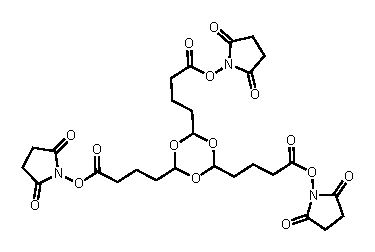
\includegraphics[scale=1.0]{figures/tri-linker.eps}
    \caption{Structure of a trioxane based trifunctional cross linker with a 
    spacer arm length of 14 {\AA}}
  \end{figure}
  DSSO has a spacer arm length of $10.1$ {\AA}.
\end{frame}
%
\begin{frame}
    \begin{figure}
    \centering
    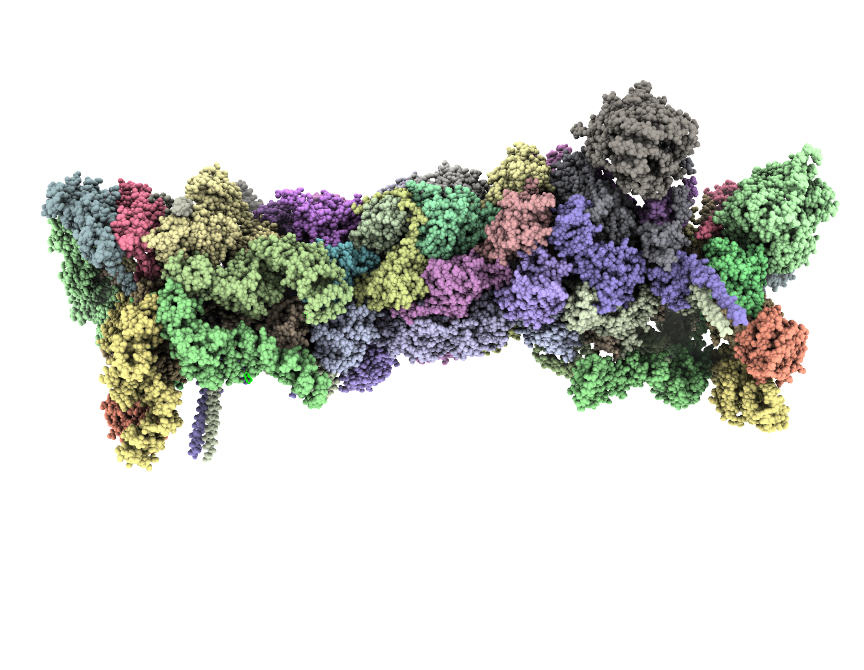
\includegraphics[width=0.5\textwidth]{figures/5gjr_structure.png}
    \caption{EM structure at 3.5 {\AA} resolution of the human 26S proteasome, PDB ID: 5GJR}
    \end{figure}
    % a table with two rows and two columns
\begin{table}
    \centering
    \caption{Number of unique cross links}
    \begin{tabular}{|c|c|}
        \hline
        Type of XL & Number of unique XLs \\ \hline
        Triple & 35 \\ \hline
        Double & 491 \\ \hline
    \end{tabular}
\end{table}
\end{frame}
%
\begin{frame}
    \frametitle{Working with the base subcomplex}
\begin{figure}
\centering
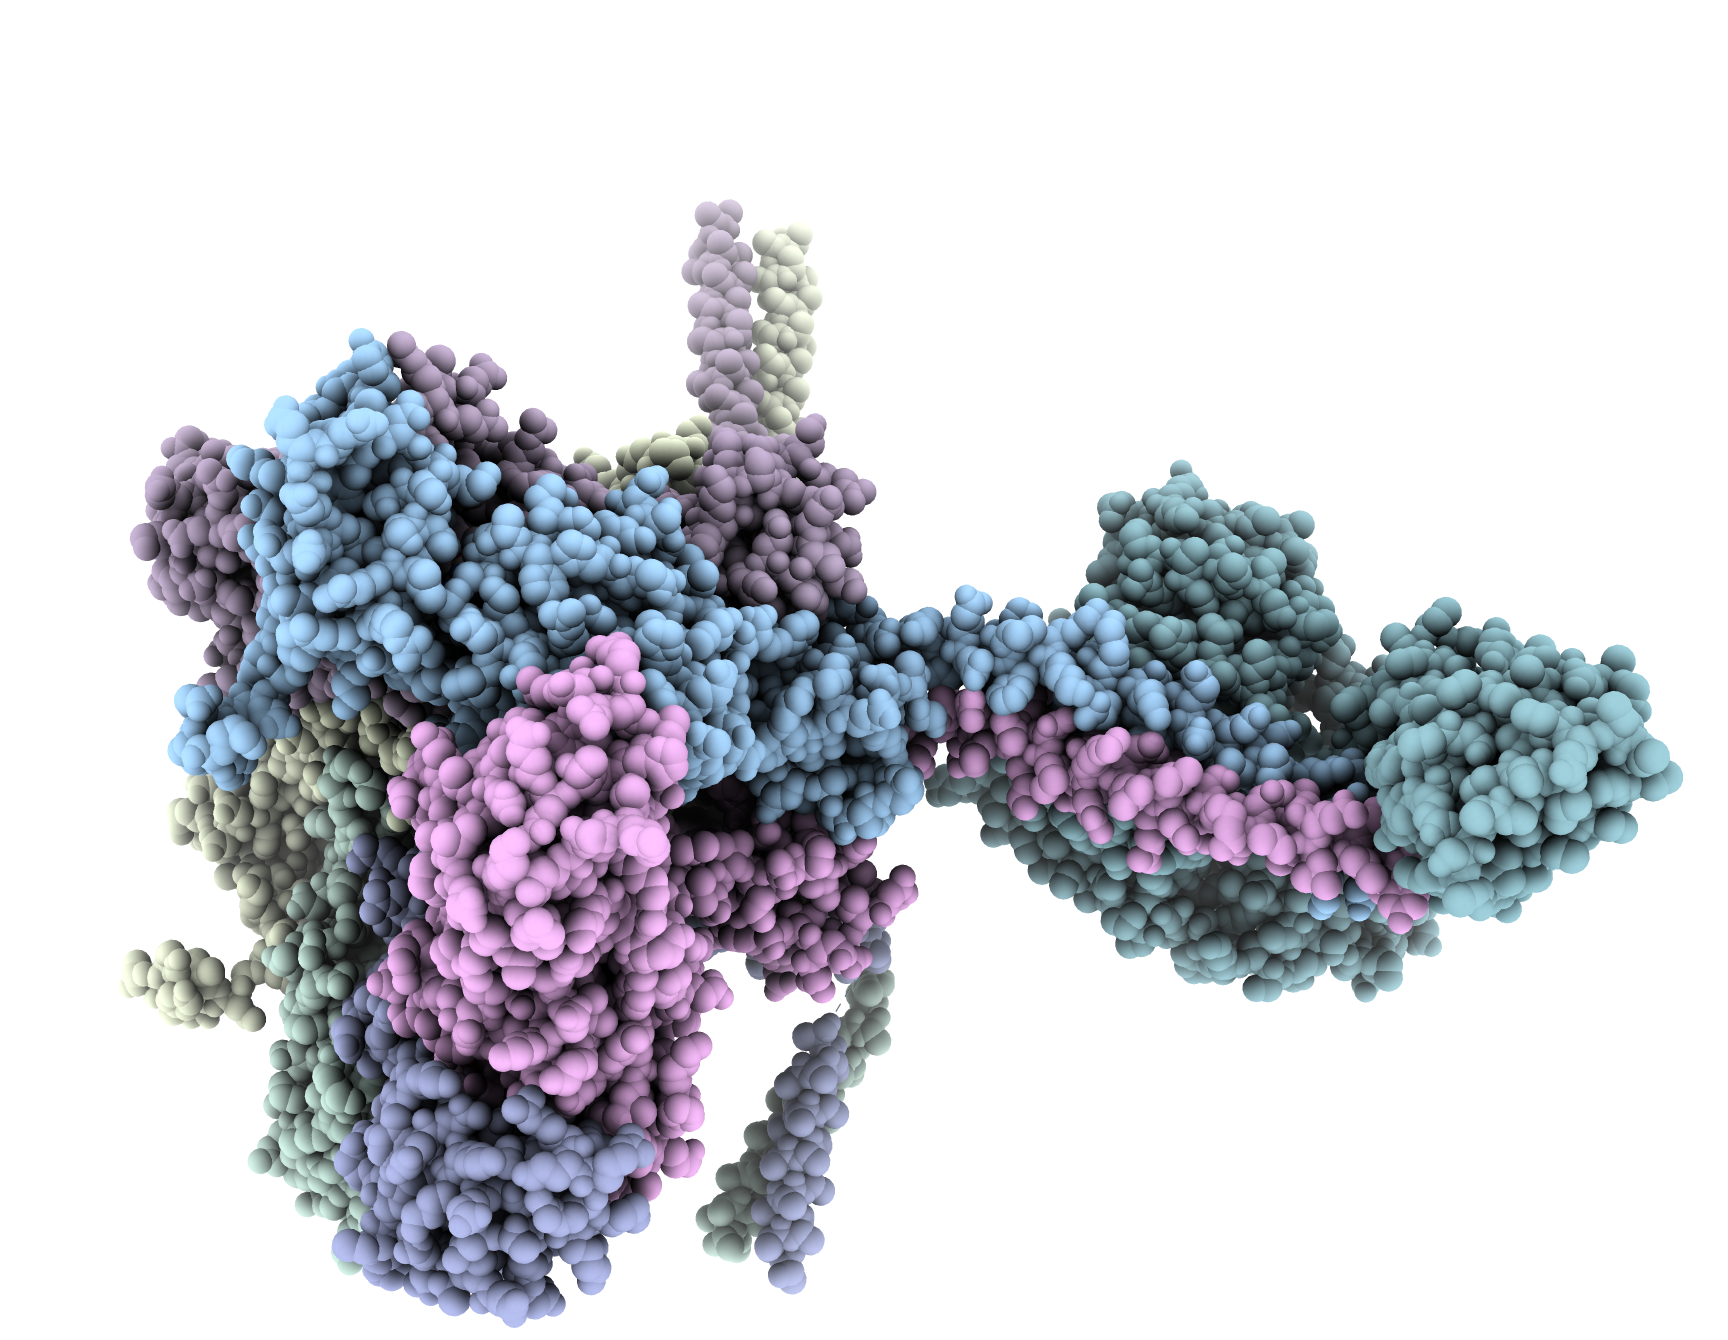
\includegraphics[width=0.5\textwidth]{figures/base_proteasome_5gjr.png}
\caption{Base subcomplex consisting of Rpt1, Rpt2, Rpt3, Rpt4, Rpt5, Rpt6, Rpn2 of subunits 
of the human 26S proteasome}
  \end{figure}
\end{frame}
%
\begin{frame}
  \begin{figure}
    \centering
    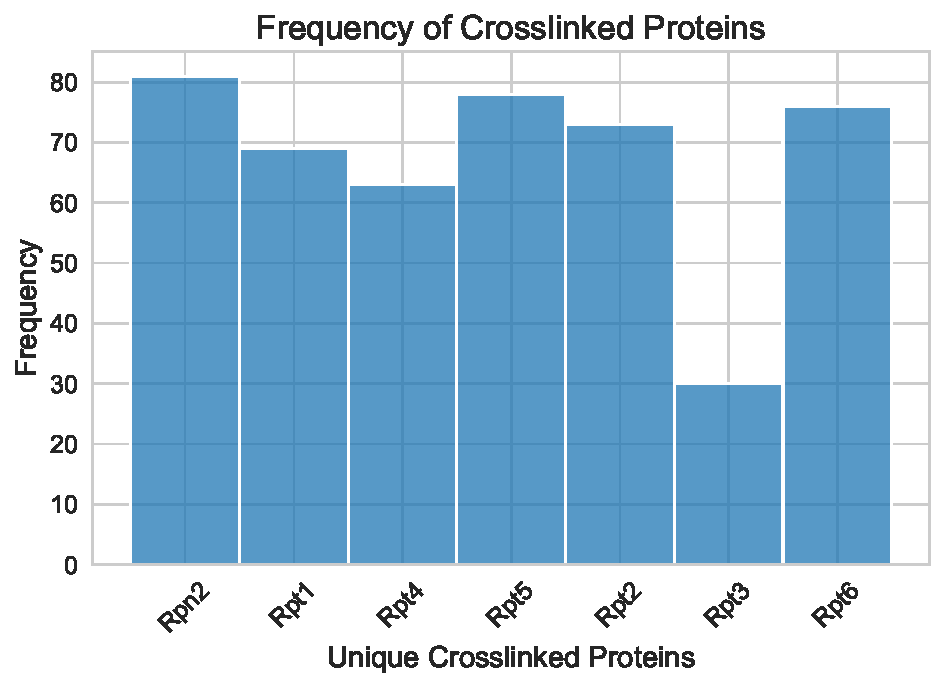
\includegraphics[width=0.6\textwidth]{figures/xl_density.pdf}
    \caption{Trifunctional cross linking mass spectrometry data}
  \end{figure}
\end{frame}
%
\begin{frame}
    \begin{figure}
    \centering
    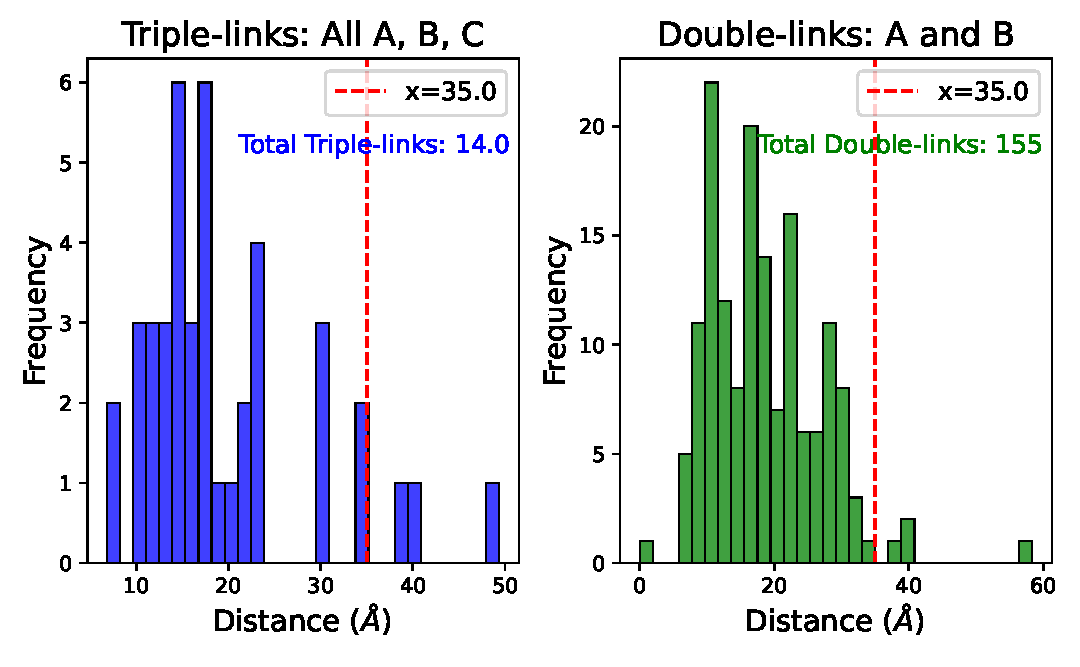
\includegraphics[width=0.6\textwidth]{figures/xls_satisfaction_base.pdf}
    \caption{Double and triple cross linked residues mapped onto the pdb strucutre 5GJR}
    \end{figure}
    \begin{itemize}
        \item Total number of double XLs: 214, out of which 59 entries had 
        residues that are not part of the 5GJR pdb structure
        \item Total number of triple XLs: 14 and all the residues are part 
        of the pdb structure
    \end{itemize}
\end{frame}
%
\end{document}
